\documentclass{article}

\usepackage{fontspec}
\usepackage{polyglossia}
\usepackage{notomath}
\setmainfont{GFS Artemisia}
\setsansfont{Source Code Pro}
\setmonofont{Source Code Pro}
\newfontfamily\greekfont[Script=Greek]{GFS Artemisia}
\newfontfamily\greekfontsf[Script=Greek]{GFS Artemisia}
\newfontfamily\greekfonttt[Script=Greek]{Source Code Pro}

%languages
\setdefaultlanguage{greek}
\setotherlanguages{english}


%typing
\usepackage{hyphenat}
\usepackage{float}
\usepackage{color, colortbl}
\usepackage{placeins}

%captions
\usepackage{caption}
\usepackage{subcaption}

%bib
% \usepackage{biblatex}
% \addbibresource{bib.bib}

%gemoetry
\usepackage[a4paper,top=1.2cm,bottom=1.2cm,left=1.2cm,right=1.2cm,marginparwidth=1.5cm]{geometry}

%images
\usepackage{graphicx}
\usepackage{tikz}

%ref
\usepackage[colorlinks=true, allcolors=blue]{hyperref}


\usepackage[export]{adjustbox}

%label
\usepackage{enumitem}
\renewcommand{\labelenumii}{\arabic{enumi}.\arabic{enumii}}
\renewcommand{\labelenumiii}{\arabic{enumi}.\arabic{enumii}.\arabic{enumiii}}
\renewcommand{\labelenumiv}{\arabic{enumi}.\arabic{enumii}.\arabic{enumiii}.\arabic{enumiv}}

%columnnew
\newcolumntype{g}{>{\columncolor{gray}}l}

%colors
\usepackage[dvipsnames]{xcolor}
\definecolor{gray}{gray}{0.9}
\definecolor{blue}{RGB}{82, 138, 174}
\definecolor{green}{RGB}{140, 219, 169}
\definecolor{yellow}{RGB}{253, 221, 92}

% \usepackage{titling}
% \setlength{\droptitle}{-20em}             %allagh glwssas
\hypersetup{
    colorlinks = true,
    linkcolor=black}


\usepackage{autobreak}


%Customize tables
\renewcommand{\arraystretch}{1.2}
% \rowcolors{2}{gray}{white}



\captionsetup[table]{
    format=plain,
    labelfont={small,it,bf}, % Small, italic, and bold label
    textfont={small,it}, % Italic text
    labelsep=colon % Colon separator
}



% Customize the figure caption
\captionsetup[figure]{
    format=plain,
    labelfont={small,it,bf}, % Small, italic, and bold label
    textfont={small,it}, % Italic text
    labelsep=colon % Colon separator
}

\makeatletter
\renewcommand*{\p@table}{\textit{Πίν. }}
\renewcommand*{\p@figure}{\textit{Σχ. }}
\renewcommand*{\p@equation}{\textit{Εξ. }}
\makeatother

\begin{document}
%TITLE
\newcommand{\uni}{ΑΡΙΣΤΟΤΕΛΕΙΟ ΠΑΝΕΠΙΣΤΗΜΙΟ ΘΕΣΣΑΛΟΝΙΚΗΣ}
\newcommand{\faculty}{ΠΟΛΥΤΕΧΝΙΚΗ ΣΧΟΛΗ}
\newcommand{\tmhma}{ΤΜΗΜΑ ΜΗΧΑΝΟΛΟΓΩΝ ΜΗΧΑΝΙΚΩΝ}


\newcommand{\titlos}{Δυναμικά φαινόμενα}
\newcommand{\ypotitlos}{Bonus Εργασία - Ειδικά Κεφάλαια Πεπερασμένων Στοιχείων}


\newcommand{\onomaauthor}{ΒΑΣΙΛΕΙΟΣ ΠΑΠΑΜΙΧΑΗΛ}


\newcommand{\advisor}{Γάκιας Χρήστος}
\newcommand{\mailauthor}{\href{mailto:vasilepi@meng.auth.gr}{vasilepi@meng.auth.gr}}
\newcommand{\aem}{6920}
\newcommand{\hmeromhnia}{\today}



\begin{titlepage}
    \begin{center}
    \raisebox{20mm}{
    \begin{tikzpicture}
        \draw (0,0) -- (6,0);
    \end{tikzpicture}}
\includegraphics[width=4cm]{media/autheng.jpg}\raisebox{20mm}{\begin{tikzpicture}
        \draw (0,0) -- (6,0);
    \end{tikzpicture}}
     \end{center}
    
    \begin{center}
        \large
        \uni\\
        \normalsize
        \faculty\\
        \vspace{1em}
        \tmhma
    \end{center}

    \vspace{2cm}
    \begin{center}
        \Large
        \textbf{\titlos}\\
        \vspace{1em}
        \large
        \textit{\ypotitlos}
    \end{center}
    \begin{center}
        \begin{tikzpicture}
        \draw (0,0) -- (4,0);
    \end{tikzpicture}\\
    \vspace{7em}
    \Large
    \textcolor{BrickRed}{\textbf{\onomaauthor}}\\
    \vspace{3em}
    
\includegraphics[width=0.3\textwidth]{media/newlogov3-cropped-content.png}
    \end{center}

    \vspace{7em}
    \hspace{4ex}
    \begin{minipage}[t]{0.45\textwidth} 
        \raggedright
        \textbf{Υπεύθυνος}: \advisor\\
        \textbf{Email}: \mailauthor\\
        \textbf{ΑΕΜ}: \aem
    \end{minipage}\\

    \vspace{4cm}
    \begin{center}
        \textit{\hmeromhnia}\\
        \begin{tikzpicture}
            \draw (0,0) -- (15,0);
        \end{tikzpicture}
    \end{center}
    
    
\end{titlepage}
\tableofcontents
%MAIN BODY

\section{Εισαγωγή}
\subsection{Παρουσίαση προβλήματος}

Στη παρόν εργασία μελετάται η ελαστοπλαστική συμπεριφορά υλικού τόσο σε κυκλική φόρτιση όσο και σε καθαρό εφελκυσμό. Σκοπός είναι, η αναπαργωγή των πειραματικών δεδομένων του υλικού και πιο συγκεκριμένα της καμπύλης τάσης παραμόρφωσης μονοτονικής συμπεριφοράς αλλά και των βρόγχων υστέρησης, δηλαδή της σταθεροποιημένης καμπύλης υλικού κυκλική συμπεριφοράς. Η όλη μελέτη γίνεται σε κύβο $10\times 10\times 10\; mm$ διαστάσεων που φορτίζεται εφελκυστικά. 
\par Η επιλογή του υλικού ήταν ανοιξείδωτος χάλυβας 316L σύμφωνα με την \cite{RASMUSSEN200347}. Στη συγκεκριμένη μελέτη δίνονται οι σταθερές κυκλικής συμπεριφοράς για διάφορα δοκίμια του υλικού. Παρακάτω φαίνονται οι σταθερές του υλικού που ακολουθούν το μοντέλο:
\begin{equation}
    \epsilon = \frac{\sigma}{E_0} + 0.002 \bigg(\frac{\sigma}{\sigma_{0.2}} \bigg)^n
\end{equation}
Τα δεδομένα που επιλέχθηκαν ήταν προφανώς μόνο για δοκίμια πάχους 10 χιλιοστών ενώ για τη μοντελοποίηση έπειτα χρησιμοποιήθηκαν οι average τιμές.
\begin{table}[H]
    \centering
    \rowcolors{2}{gray}{white}
        \begin{tabular}{|c|c|c|c|c|c|c|c|c|}
        \hline
        \rowcolor{Dandelion}
        Spec. \# & $t\; [mm]$ & l. rate & $\sigma_{0.2}\; [MPa]$ & $\sigma_{1.0}\; [MPa]$ & $\sigma_u\; [MPa]$ & elong \% & $E_0 \; [GPa]$ & n\\
        \hline
        LT1R & 10 & 3 & 252.8 & 296.3 & 585.7 & 50 & 185.5 & 7.9 \\
        \hline
        LT2R & 10 & 0.3 & 244.7 & 288.6 & 586.5 & 47 & 187.8 & 7.9 \\
        \hline
        LT3R & 10 & 30 & 265.1 & 307.4 & 584.8 & 52 & 195.4 & 5.8 \\
        \hline
        LT4R & 10 & 3 & 262.6 & 303.6 & 588.1 & 48 & 194.6 & 7.5 \\
        \hline
        LT5R & 10 & 0.3 & 248.1 & 291.1 & 590.3 & 49 & 189.4 & 9.8 \\
        \hline
        LT6R & 10 & 30 & 295.6 & 319.7 & 588.9 & 48 & 200.1 & 6.7 \\
        \hline
        LT7R & 10 & 3 & 260.6 & 295.3 & 579.5 & 52 & 196.9 & 8.8 \\
        \hline
        Average & 10 & - & 272.5 & 311.3 & 583.9 & 47.9 & 192.8 & 7.1 \\
        \hline
        \end{tabular}
    \caption{Πειραματικά αποτελέσματα 316L υπό εφελκυστική φόρτιση.}
    \label{tab:peiram}
\end{table}
Ζητούνται πιο συγκεκριμένα:

\begin{itemize}
\item Θα δημιουργήσετε έναν κύβο διαστάσεων 10x10x10 mm και θα τον
διακριτοποιήσετε με τουλάχιστον 3 στοιχεία σε κάθε διαστασή του.
\item Θα εφαρμόσετε κατάλληλες οριακές συνθήκες ώστε να φορτίζεται σε καθαρό
εφελκυσμό.
\item Υπό εφελκυστική φόρτιση, θα εξεταστεί η ελαστοπλαστική συμπεριφορά,
ακολουθώντας τις εξής παραδοχές:
\begin{itemize}
\item Τέλεια πλαστική συμπεριφορά
\item Γραμμική κράτυνση
\item Εκθετική κράτυνση (δημιουργώντας καμπύλη με πολλά σημεία)
\end{itemize}
Θα πρέπει να αναπαράγετε με τη μέγιστη δυνατή ακρίβεια για κάθε παραδοχή, τα
δεδομένα του υλικού που έχετε επιλέξει. Επίσης, θα πρέπει να εξετάσετε τις
παραμέτρους προεκβολής που δίνει ως επιλογή ο επιλυτής.
\item Υπό εναλλασσόμενη φόρτιση θα εξετάσετε την σταθεροποιημένη κυκλική
συμπεριφορά του υλικού, ακολουθώντας της εξής παραδοχές:
\begin{itemize}
\item Ισοτροπική κράτυνση, σε συνδυασμό με τις παραδοχές ελαστοπλαστικής
συμπεριφοράς του ερωτήματος 3.
\item Κινηματική κράτυνση, σε συνδυασμό με τις παραδοχές ελαστοπλαστική
συμπεριφοράς του ερωτήματος 3.
\item Η κυκλική συμπεριφορά θα πρέπει να εξεταστεί στην περίπτωση ελέγχου
δύναμης και ελέγχου μετατόπισης.
\end{itemize}
Θα πρέπει να αναπαράγετε με τη μέγιστη δυνατή ακρίβεια για κάθε παραδοχή, τα
δεδομένα του υλικού σε κυκλική φόρτιση που έχετε επιλέξει.
\item Να εξετάσετε παραμέτρους του επιλυτή που αφορούν την αστοχία του υλικού σε
κάποια μέγιστη τιμή τάσης ή/και παραμόρφωσης.
\item Θα πρέπει να είστε σε θέση να ποσοτικοποιήσετε τις αποκλίσεις που θα
παρατηρήσετε καθώς και να τις εξηγήσετε κατάλληλα.
\item Οποιοδήποτε φαινόμενο παρατηρήσετε στα αποτελέσματά σας, θα πρέπει να το
χαρακτηρίσετε και να το εξηγήσετε με τις κατάλληλες βιβλιογραφικές αναφορές.
\item Είστε ελεύθεροι να χρησιμοποιήσετε οποιαδήποτε άλλη παράμετρο προσφέρει ο
επιλυτής.
\end{itemize}

\section{Μοντελοποίηση}

\subsection{Μονοτονική συμπεριφορά}
Όσο αναφορά τη μονοτονική συμπεριφορά, δημιουργείται κύβος με 5 στοιχεία σε κάθε ακμή. Για τις οριακές συνθήκες, ώστε νε επιτευχθεί καθαρός εφελκυσμός, η μια πλευρά του κύβου περιορίζεται στον άξονα εφαρμογής της δύναμης, στο ίδιο επίπεδο που βρίσκεται αυτή η επιφάνεια περιορίζονται δύο ακμές του κύβου στους άλλους δύο άξονες (με τις ακμές να είναι κάθετες στον άξονα στον οποίο περιορίζονται). Γίνεται πιο εύκολα αντιληπτό και από το \ref{fig:bcs}. Οι ίδιες οριακές συνθήκες χρησιμοποιήθηκαν προφανώς και για τη θράυση αλλά και για τη κυκλική φόρτιση.

\begin{figure}[H]
    \centering
    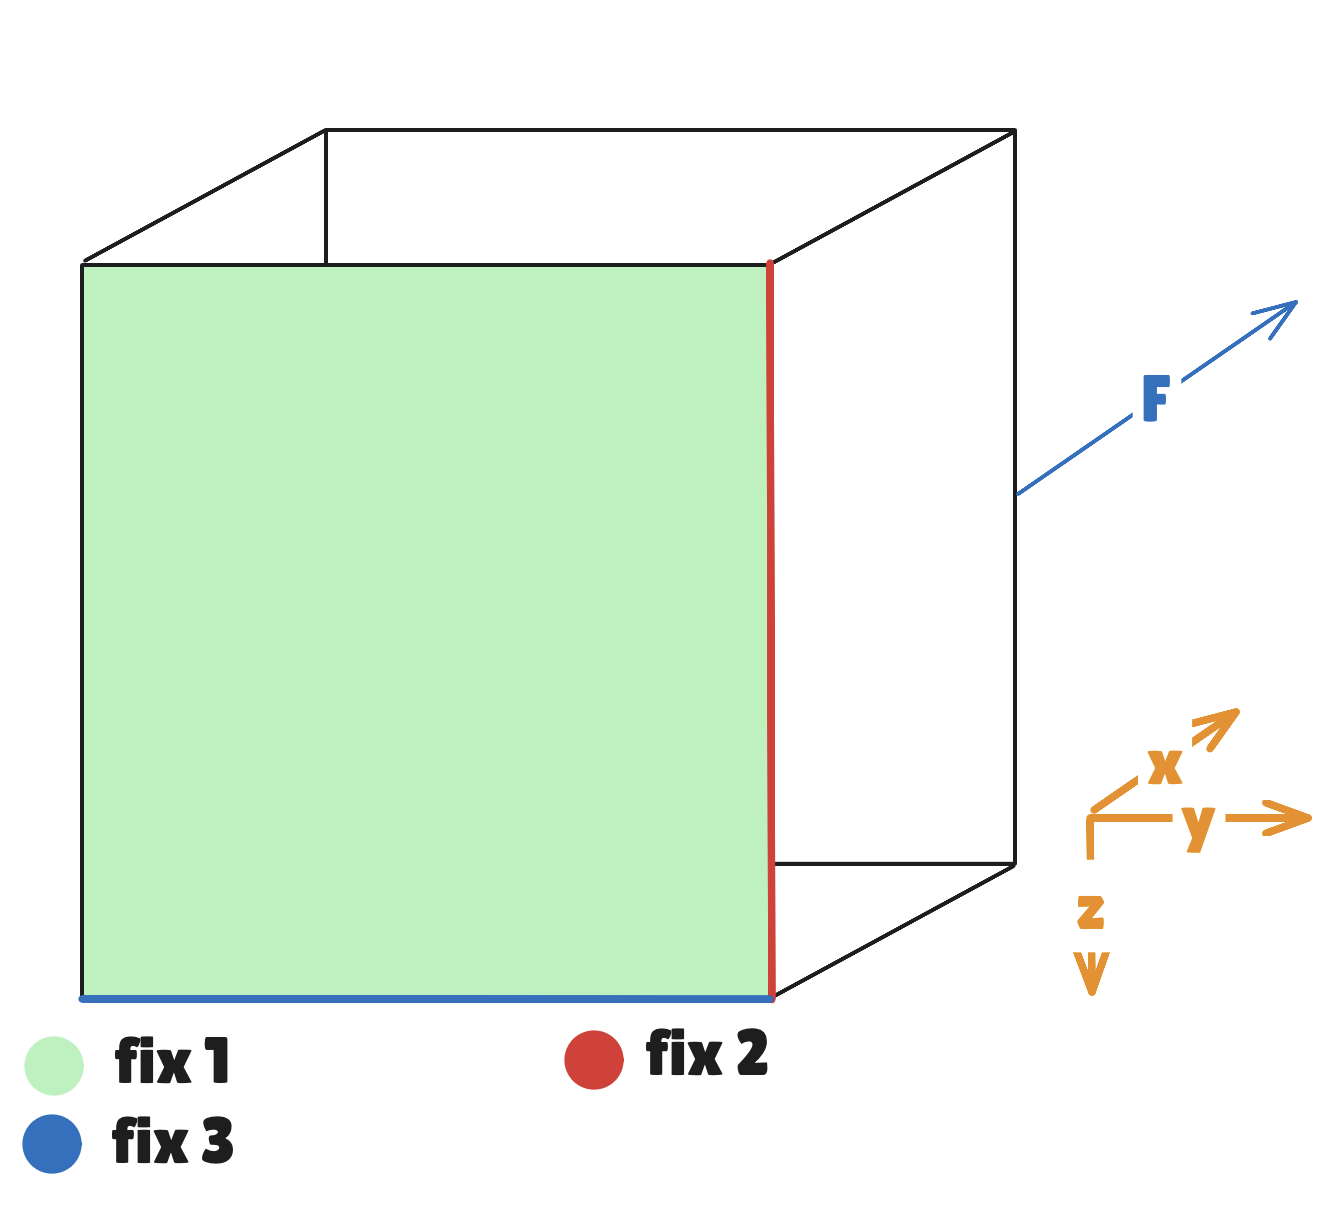
\includegraphics[width=0.7\linewidth]{media/bcs.png}
    \caption{Οριακές συνθήκες για επίτευξη καθαρού εφελκυσμού κύβου.}
    \label{fig:bcs}
\end{figure}

Επίσης, για μεγαλύτερη σταθερότητα κατά την επίλυση, χρησιμοποιήθηκε μετατόπιση και όχι φορτίο ώστε να επιτευχθεί η παραμόρφωση του κύβου. Η μετατόπιση που πρέπει να δωθεί στην επιφάνεια του κύβου είναι προφανώς $u = \epsilon_{max} \cdot 10$, ώστε να φτάσει το υλικό αυτή τη παραμόρφωση που εμφανίζεται και στην Ramberg-Osgood. Η μέγιστη παραμόρφωση  υπολογίζεται από την Ramberg-Osgood αναλυτικά έως την τάση $\sigma_u$ του υλικού, δηλαδή $\epsilon_{max} = \epsilon_u$. 
\par Για τον ορισμό της πλαστικότητας του υλικού ορίζονται πίνακες πλαστικότητας σύμφωνα με τις προδιαγραφές του επιλυτή. Παρακάτω φαίνονται τα αναλυτικά αποτελέσματα καθώς και μόνο η πλαστική παραμόρφωση του υλικού, δηλαδή οι τιμές εισαγωγής στον επιλυτή.
\begin{figure}[H]
    \centering
    \begin{subfigure}{0.45\linewidth}
        \centering
        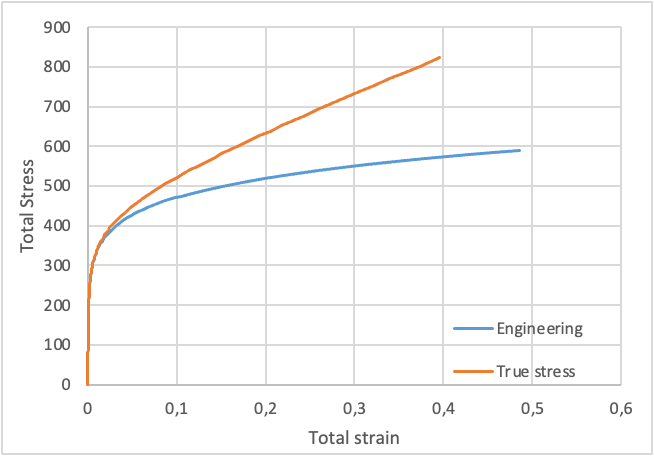
\includegraphics[width=\linewidth]{media/ragood.png}
        \caption{Αναλυτική καμπύλη Ramberg-Osgood 316L.}
        % \label{fig:label1}
    \end{subfigure}
    \hfill
    \begin{subfigure}{0.45\linewidth}
        \centering
        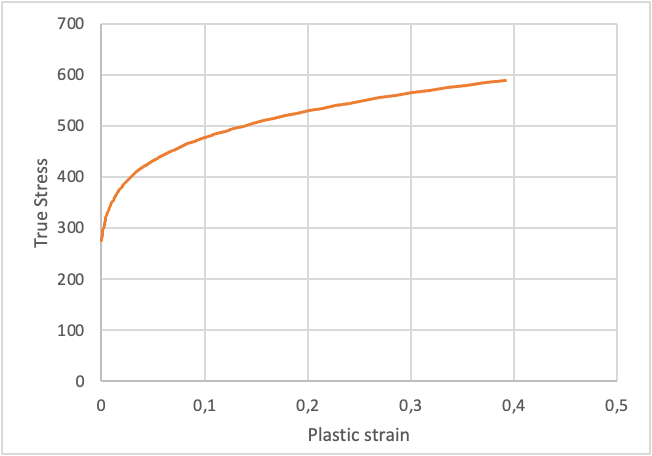
\includegraphics[width=\linewidth]{media/plabaqus.png}
        \caption{Πλαστική παραμόρφωση 316L.}
        % \label{fig:label2}
    \end{subfigure}
    \caption{Αναλυτικές καμπύλες μονοτωνικής συμπεριφοράς ανοιξείδωτου χάλυβα 316L.}
    \label{fig:anal}
\end{figure}
Για τις επιλύσεις τέλειας πλαστικότητας και γραμμικής πλαστικότητας δίνονται μόνο το πρώτο σημείο της καμπύλης πλαστικής παραμόρφωσης και το πρώτο και τελευταίο σημείο της καμπλύλης αντίστοιχα. 
\par Όσο αναφορά την κατάστρωση της επίλυσης, είναι πολύ σημαντική η επιλογή του βήματος επίλυσης. Στην αρχή η επίλυση έγινε με \texttt{TIME INC} = 0.1 και αποδείχθηκε, ότι δεν προσαρμόζεται σωστά η αριθμητική καμπύλη στο μέτρο ελαστικότητας του υλικού. Έτσι, το μοντέλο επιλύεται δεύτερη φορά με μικρότερο βήμα.
\begin{figure}[H]
    \centering
    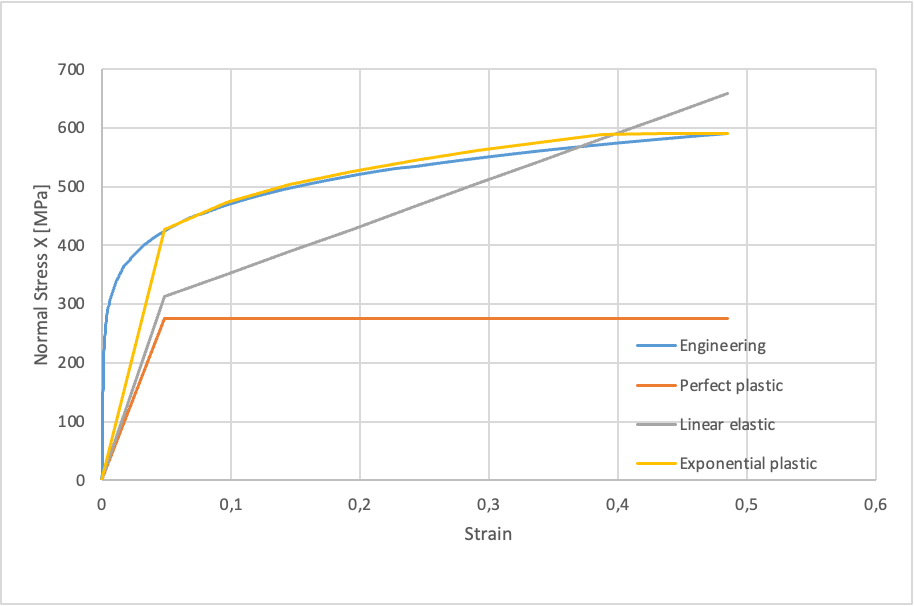
\includegraphics[width=0.8\linewidth]{media/static-false.png}
    \caption{Μη καλή προσέγγιση μονοτονικής συμπερφοράς λόγω μεγάλου βήματος επίλυσης.}
    \label{fig:statfalse}
\end{figure}

\subsection{Κυκλική συμπεριφορά}
Για την επίλυση της κυκλικής φόρτισης, γίνεται πιο πυκνό πλέγμα με 8 στοιχεία σε κάθε ακμή ώστε να επιτευχθεί πιο σταθερή λύση.

















\listoffigures
\listoftables

\nocite{*}
\printbibliography

\end{document}